% !TeX spellcheck = id_ID
\documentclass[a4paper,12pt]{article}
\usepackage[bahasa]{babel}
\usepackage{graphicx}
\usepackage{multirow}
\usepackage{enumitem}
\usepackage{listings}
\graphicspath{ {./img/} }
\begin{document}
\title{Taksonomi Flynn}
%\author{Aldzikri Dwijayanto Prathama \\ {\small 195410189}}
\author{Aldzikri Dwijayanto Prathama 
	\\195410189}
\makeatletter
\begin{titlepage}
	\begin{center}
		{\huge \bfseries \@title }\\[14ex]
		
\includegraphics[scale=.8]{logo}\\[4ex]
		{\large \@author}\\[20ex]
		{\large \bfseries {SEKOLAH TINGGI MANAJEMEN INFORMATIKA DAN KOMPUTER
				AKAKOM YOGYAKARTA}}
	\end{center}


%{\large \@date} 
\end{titlepage}
\makeatother
%\maketitle
\newpage
\tableofcontents
\newpage
\section{Taksonomi Flynn}
Taksonomi Flynn, dalam arsitektur komputer, adalah sebuah klasifikasi yang dibuat oleh Michael J. Flynn pada tahun 1966. Klasifikasi ini dibuat berdasarkan jumlah instruksi yang berjalan simultan dan konkuren, dan juga aliran data yang diprosesnya. Dalam Taksonomi Flynn, komputer dibagi menjadi empat buah kelas, yakni
\begin{itemize}
    \item Single Instruction Single Data Stream (SISD)
    \item Single Instruction Multiple Data Stream (SIMD)
    \item Multiple Instruction Single Data stream (MISD)
    \item Multiple Instruction Multiple Data Stream (MIMD)
\end{itemize}

\subsection{Single Instruction Single Data Stream (SISD)}

Single Instruction Single Data Stream (SISD), yaitu sebuah komputer yang tidak memiliki cara untuk melakukan paralelisasi terhadap instruksi atau data. Contoh mesin SISD adalah PC tradisional atau mainframe yang tua.
\begin{center}
    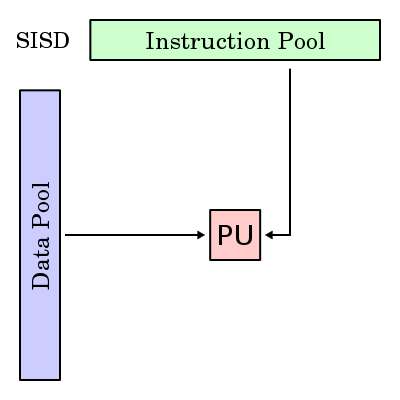
\includegraphics[width=0.8\linewidth]{sisd.png}
\end{center}
Instruksi dilaksanakan secara berurut tetapi jugaboleh overlap dalam tahapan eksekusi (pipeline)
Satu alur instruksi didecode untuk alur data tunggal
Contoh mesin SISD adalah PC tradisional atau mainframe yang tua, yang hanya bisa melakukan single instruksi/tunggal

\subsection{Single Instruction Multiple Data Stream (SIMD)}
Single Instruction, Multiple Data Stream (SIMD), yaitu sebuah komputer yang mampu memproses banyak aliran data dengan hanya satu instruksi, sehingga operasi yang dilakukan adalah operasi paralel. Contoh dari SIMD adalah prosesor larik (array processor), atau GPU.
\begin{center}
    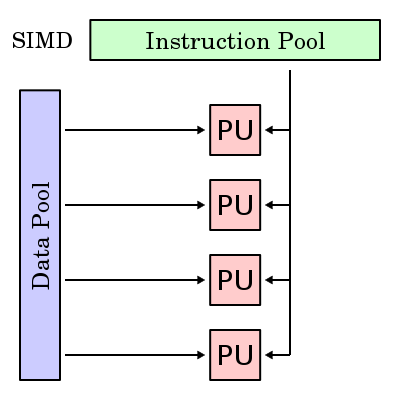
\includegraphics[width=0.8\linewidth]{simd.png}
\end{center}
Beberapa Processor Unit (ProcessingElement) disupervisi oleh Control Unityang sama.
Semua Processing Element menerimainstruksi yang sama dari control unit tetapimengeksekusi data yang berbeda dari alurdata yang berbeda pula.
Subsistem memori berisi modul-modul memori.
Processor vektor dan processor arraytermasuk dalam kategori ini.

\subsection{Multiple Instruction Single Data stream (MISD)}
Multiple Instruction, Single Data Sream (MISD), yaitu sebuah komputer yang dapat melakukan banyak instruksi terhadap satu aliran data. Komputer ini, tidak memiliki contoh, karena meski pernah dibuat, hal itu dibuat sebagai purwarupa (prototipe), dan tidak pernah dirilis secara massal.
\begin{center}
    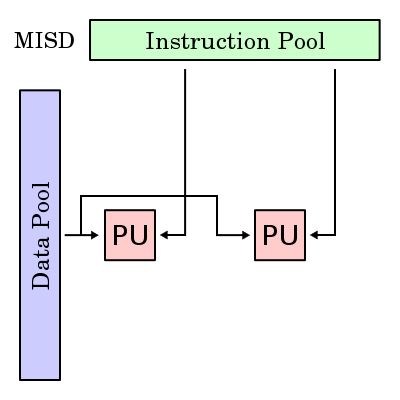
\includegraphics[width=0.8\linewidth]{misd.png}
\end{center}
Sejumlah PU , masing-masing menerima instruksi yang berbeda danmengoperasikan data yang sama.
Output salah satu prosesor menjadi inputbagi prosesor berikutnya.
Struktur komputer ini tidak praktis,sehingga tidak ada komputer yang menggunakannya.

\subsection{Multiple Instruction Multiple Data Stream (MIMD)}
Multiple Instruction, Multiple Data stream (MIMD), yaitu sebuah komputer yang memiliki beberapa prosesor yang bersifat otonomus yang mampu melakukan instruksi yang berbeda pada data yang berbeda. Sistem terdistribusi umumnya dikenal sebagai MIMD, entah itu menggunakan satu ruangan memori secara bersama-sama atau sebuah ruangan memori yang terdistribusi.
\begin{center}
    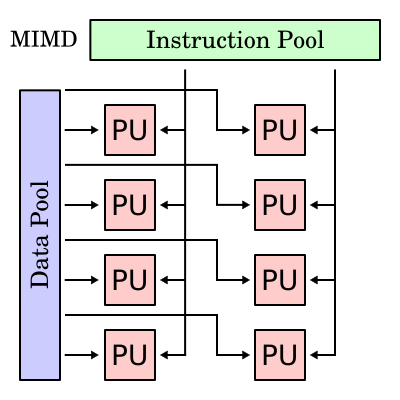
\includegraphics[width=0.8\linewidth]{mimd.png}
\end{center}
Sejumlah prosesor secara simultanmengeksekusi rangkaian instruksi yangberbeda pada kumpulan data yangberbeda pula.
MIMD dapat berupa multiprosesor denganmemori yang dapat digunakan bersama(shared memory) atau multikomputerdengan memori yang terdistribusi

\end{document}
